% === T06 - Microarquitectura (uArch) ===
% David Alejandro Gonzalez Marquez
% fokerman@gmail.com
% https://github.com/fokerman/fpgaSoftcoreProgrammingCourse

\RequirePackage[2020-02-02]{latexrelease}

\documentclass[aspectratio=169]{beamer}
\usepackage{../packages}

\newcommand{\na}{\cellcolor{naranjauca}}
\newcommand{\gm}{\cellcolor{gray!50}} 

\title{\Huge Microarquitectura (uArch)}
\author{David Alejandro González Márquez}
\institute{Programación de softcores en FPGAs\\
Programa de Profesoras/es Visitantes\\
Departamento de computación\\
Universidad de Buenos Aires}


\date{}

\begin{document}

\begin{frame}[plain]
    \titlepage
    \begin{textblock}{110}(25,80)
    \begin{tcolorbox}[size=small,width=\textwidth,colback={gray!30},title={}]
    \begin{center}
     \scriptsize Clase disponible en: \url{https://github.com/fokerman/fpgaSoftcoreProgrammingCourse}
    \end{center}
    \end{tcolorbox}
    \end{textblock}
\end{frame}

\begin{frame}[t,fragile]
    \frametitle{Microarquitectura}
    La \textbf{microarquitectura} de un procesador hace referencia a su diseño interno.\\
    \textcolor{verdeuca}{Usualmente denominada la \textbf{organización} del procesador.}\\
    \bigskip
    \pause
    \bigskip
    En esta clase vamos a presentar una \textbf{implementación de la arquitectura MIPS}.\\
    \bigskip
    \pause
    Primero proponiendo un diseño simple donde se presenten las técnicas utilizadas para pensar y construir un \emph{datapath}.
    \pause
    \textcolor{verdeuca}{El objetivo es diseñar un sistema que responda al procesamiento de instrucciones, buscando ejecutarlas lo \textbf{más rápido posible}.}
    \textcolor{naranjauca}{\textbf{En un solo ciclo de reloj}.}\\
    \bigskip
    \pause
    Para luego extender está solución aplicando la \textbf{técnica de segmentación} o \textcolor{naranjauca}{\textbf{\emph{pipeline}}}.\\
    \pause
    \textcolor{verdeuca}{Donde nos vamos a encontrar con múltiples problemas derivados de separar en partes las instrucciones.}
\end{frame}

\begin{frame}[t,fragile]
    \frametitle{Arquitectura MIPS}
    \footnotesize
    Tamaño de palabra de 32 bits, con instrucciones de 32 bits.\\
    32 registros en total entre dedicados y propósito general.\\
    \uncover<2->{\textcolor{verdeuca}{Tres tipos de codificación de instrucciones.}}
    \begin{textblock}{100}(13,28)
    \includegraphics[scale=0.73]{imgBook/reference_MIPS_registers.pdf}
    \end{textblock}
    \begin{textblock}{100}(8,70)
    \uncover<2->{
\includegraphics[scale=0.73]{imgBook/reference_MIPS_formats.pdf}}
    \end{textblock}
    \begin{textblock}{100}(88,3)
    \uncover<3->{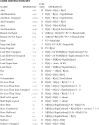
\includegraphics[scale=0.67]{imgBook/reference_MIPS_instructions.pdf}}
    \end{textblock} 
\end{frame}

\begin{frame}[t,fragile]
    \frametitle{Implementación básica de un MIPS}
    Vamos a estudiar una implementación limitada del conjunto de instrucciones de la arquitectura MIPS.\\    
    \begin{itemize}
    \item \textcolor{verdeuca}{\textbf{Instrucciones de acceso a memoria:}} \emph{load word} (\texttt{lw}), \emph{store word} (\texttt{sw})
    \item \textcolor{verdeuca}{\textbf{Instrucciones artiméticas y lógicas:}} \texttt{add}, \texttt{sub}, \texttt{AND}, \texttt{OR}, \texttt{slt}
    \item \textcolor{verdeuca}{\textbf{Instrucciones de control:}} \emph{branch equal} (\texttt{beq}), \emph{jump} (\texttt{j})
    \end{itemize}
    \pause
    \bigskip
    Estas subconjunto de instrucciones no incluye todas soportadas en la ISA.\\
    \textcolor{naranjauca}{Pero ilustra los principios de funcionamiento usados para crear y diseñar el \emph{datapath}.}\\
    \bigskip
    \textcolor{gray}{Todos los conceptos que se ilustran en está implementación son las ideas básicas que se utilizan para diseñar desde procesadores de alto rendimiento, o proposito general, hasta dispositivos embebidos.}
\end{frame}

\begin{frame}[t,fragile]
    \frametitle{Descripción general de la implementación}
    En MIPS, en general todas las instrucciones requieren pasos similares.\\
    \bigskip
    Los primeros pasos son siempre los mismos:
    \begin{enumerate}
     \item Enviar el PC a la memoria y leer el contenido (\emph{instruction fetch}).
     \item Leer uno o dos registros usando campos en la instrucción.
    \end{enumerate}
    \pause
    \bigskip
    Luego de estos dos pasos, las acciones dependen del tipo de instrucción.\\
    \vspace{0.2cm}
    Existen tres tipos de instrucciones:
    \begin{enumerate}
     \item memory-reference
     \item arithmetic-logical
     \item branches
    \end{enumerate}
    \pause
    \begin{center}
    \textcolor{verdeuca}{
    La simplicidad del conjunto de instrucciones permite que la operatoria\\
    de cada uno de los tipos de instrucciones sea similar.
    }
    \end{center}
\end{frame}

\begin{frame}[t,fragile]
    \frametitle{Vista general de la implementación}
    \begin{textblock}{100}(8,14)
    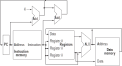
\includegraphics[scale=0.8]{imgBook/MIPS_abstract_view_F1.pdf}
    \end{textblock}
    \begin{textblock}{45}(105,8)
    \textbf{Observaciones}\\
    \small
    \begin{itemize}
    \item<2-> De la \textbf{instrucción} se toman datos para el banco de registros, el PC y la ALU.
    \item<3-> El \textbf{nuevo PC} puede provenir de dos flujos diferentes.
    \item<4-> Escribir al \textbf{banco de registros} llega desde la memoria o desde la ALU.
    \item<5-> A la \textbf{memoria} solo llegan datos del banco de registros.
    \end{itemize}
    \end{textblock}
    \begin{textblock}{140}(10,73)
    \uncover<6->{
    La ilustración indica los componentes básicos del \emph{datapath} y como se \textbf{interconectan}.\\
    \textcolor{verdeuca}{La idea es identificar especificamente el \textbf{flujo de los datos} dentro del \emph{datapat}.}
    }
    \end{textblock}
\end{frame}

\begin{frame}[t,fragile]
    \frametitle{Vista general de la implementación y líneas de control}
    \begin{textblock}{100}(50,8)
    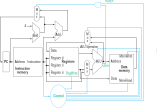
\includegraphics[scale=0.73]{imgBook/MIPS_abstract_view_control_F2.pdf}
    \end{textblock}
    \begin{textblock}{65}(8,14)
    Se agregan \textbf{líneas de\\ control},
    junto con tres\\ multiplexores.
    \small
    \begin{enumerate}
    \setlength\itemsep{0cm}
    \item<2-> Escritura en el PC.
    \item<2-> Escritura en el banco\\ de registros.
    \item<2-> Entrada a la ALU.
    \end{enumerate}
    \bigskip
    \uncover<3->{Las líneas de control toman\\ como entrada la \textbf{instrucción}.}\\
    \bigskip
    \uncover<4->{Llegan a los tres multiplexores, a la ALU,\\ al banco de registros y memoria.}\\
    \uncover<5->{\textcolor{verdeuca}{Además de una línea adicional para el control de saltos condicionales por el flag Zero.}}
    \end{textblock}
\end{frame}

\begin{frame}[t,fragile]
    \frametitle{Diseño Lógico}
    El \emph{datapath} contiene dos tipos de componentes:\\
    \begin{itemize}
     \item Componentes que dependen \textbf{solo de sus entradas} (Operación combinacional).
     \item Componentes que \textbf{mantienen un estado} (Operación secuencial).
    \end{itemize}
    \pause
    \bigskip
    Los elementos con estado soportan el comportamiento de \textbf{lectura} y \textbf{escritura}.\\
    Contienen al menos dos entradas y una salida.\\
    \pause
    \bigskip
    \textcolor{verdeuca}{
    Una de las entradas indica el dato que será escrito, y otra el clock para sincronizar el momento que de debe ser escrito.
    La salida permite obtener el dato escrito en el ciclo anterior.\\
    }
    \pause
    \bigskip
    Además de los flip-flops que respetan esté comportamiento tenemos dos tipos de elementos con estado: \textbf{Memorias} y \textbf{Registros}.\\
    \bigskip
\end{frame}
    
\begin{frame}[t,fragile]
    \frametitle{Metodología de sincronización}
    \begin{textblock}{10}(85,10)
    \includegraphics[scale=0.8]{imgBook/state_clock_F3_F4-layer1.pdf}\\
    \vspace{3cm}
    \uncover<3->{\includegraphics[scale=0.8]{imgBook/state_clock_F3_F4-layer2.pdf}}
    \end{textblock}
    \begin{textblock}{140}(10,12)
    La sincronización define cuando las señales serán\\ leídas y cuando serán escritas en función del reloj.\\
    \bigskip
    \textcolor{verdeuca}{Por simplicidad asumimos que los cambios\\ serán por flanco ascendente de reloj.}\\
    \bigskip
    \uncover<2->{
    \textcolor{gray}{
    Como solo los elementos con estado pueden guardar información, \textbf{cualquer circuito
    combinacional tiene como entradas datos provenientes de elementos con estado}.\\
    Luego, las salidas son nuevamente guardadas en otros elementos con estado.}\\
    }
    \vspace{0.8cm}
    \uncover<3->{
    Esta metodología nos permite \textbf{realimentar}\\
    la escritura de los elementos con estado\\
    por medio de un circuito combinacional.
    }
    \end{textblock}
\end{frame}

\begin{frame}[t,fragile]
    \frametitle{Construyendo un Datapath}
    Usando como guía el ciclo de instrucción. \textcolor{verdeuca}{Vamos a resolver la \textbf{etapa de \emph{fetch}}.}\\
    \begin{center}
    \includegraphics[scale=1]{imgBook/MIPS_memory_pc_adder_C4F5-layer1.pdf}
    \includegraphics[scale=1]{imgBook/MIPS_memory_pc_adder_C4F5-layer2.pdf}
    \includegraphics[scale=1]{imgBook/MIPS_memory_pc_adder_C4F5-layer3.pdf}
    \end{center}
    \pause
    La memoria contiene las instrucciones que \textbf{leemos} según indique la dirección en el PC.\\
    \bigskip
    Para pasar a la próxima instrucción debemos \textbf{incrementar} el PC usando el sumador.\\
    \bigskip
    \textcolor{verdeuca}{Ambas acciones, tanto leer de memoria y actualizar el PC se pueden realizar \textbf{en el mismo ciclo}.}\\
\end{frame}

\begin{frame}[t,fragile]
    \frametitle{Construyendo un Datapath: \emph{Fetch}}
    \begin{textblock}{100}(10,15)
    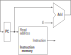
\includegraphics[scale=1]{imgBook/MIPS_datapath_PC_F6.pdf}
    \end{textblock}
    \begin{textblock}{60}(90,15)
    El PC llega tanto al puerto de direcciones de la \textbf{memoria} como al \textbf{sumador}.\\
    \bigskip
    \uncover<2->{\textcolor{verdeuca}{El sumador es un circuito combinacional que genera el nuevo PC sumandole 4 unidades.}\\}
    \bigskip
    \uncover<3->{La instrucción leída de la memoria se presenta en la \textbf{salida de la memoria} luego del ciclo de reloj.\\}
    \bigskip
    \uncover<4->{Simultáneamente el PC cambia su estado pasando a la \textbf{próxima dirección}.}
    \end{textblock}
\end{frame}

\begin{frame}[t,fragile]
    \frametitle{Construyendo un Datapath: \emph{R-format instructions}}
    \begin{textblock}{60}(90,15)
    \includegraphics[scale=0.8]{imgBook/MIPS_datapath_Reg_Alu_F7-layer1.pdf}\\
    \vspace{0.5cm}
    \uncover<4->{\includegraphics[scale=0.8]{imgBook/MIPS_datapath_Reg_Alu_F7-layer2.pdf}}
    \end{textblock}
    \begin{textblock}{100}(10,15)
    Las instrucciones \emph{R-format} operan con tres registros.\\ \textcolor{verdeuca}{Dos como entrada y uno como salida.}\\
    \uncover<2->{\textcolor{gray}{En un banco de registros se puede seleccionar\\ cualquiera de los registros para ser \textbf{escrito o leído}.}\\}
    \bigskip
    \uncover<3->{Los puertos de lectura permiten seleccionar\\ simultáneamente dos registros para ser leídos.\\}
    \bigskip
    \uncover<4->{
    \textcolor{verdeuca}{
    Los datos leídos \textbf{entran} como parámetros directamente en\\
    la ALU que realiza la operación seleccionada y genera un\\
    resultado que es almacenado nuevamente en el banco de\\ registros.}\\}
    \bigskip
    \uncover<5->{MIPS cuenta con 32 registros ($2^5$), y cada registro es de 32 bits.}
    \end{textblock}
\end{frame}

\begin{frame}[t,fragile]
    \frametitle{Construyendo un Datapath: \emph{load/store instructions}}
    \begin{textblock}{60}(110,15)
    \includegraphics[scale=0.8]{imgBook/MIPS_memory_signExt_C4F8-layer1.pdf}\\
    \vspace{0.5cm}
    \uncover<3->{\includegraphics[scale=0.8]{imgBook/MIPS_memory_signExt_C4F8-layer2.pdf}}
    \end{textblock}
    \begin{textblock}{95}(10,15)
        Las instrucciones \emph{load}/\emph{store} son de la forma:
        \begin{itemize}
        \item \textcolor{naranjauca}{LOAD}: \hspace{0.28cm} \verb|lw $t1, offset_value($t2)|
        \item \textcolor{naranjauca}{STORE}:\hspace{0.2cm} \verb|sw $t1, offset_value($t2)|
        \end{itemize}
        \bigskip
        \uncover<2->{
        \textcolor{verdeuca}{
        El primer parámetro es un registro fuente o destino del dato.\\
        El segundo parámetro es un registro más un offset de 16 bits.\\
        }}
        \bigskip
        \uncover<3->{Para poder operar con el offset de manera signada se tiene un\\
        componente que extiende el signo a 32 bits.\\}
        \bigskip
        \uncover<4->{
        \textcolor{gray}{
        La codificación de los registros en cada caso es la misma.\\
        \textbf{Las señales de control indican si se trata de una lectura o escritura.}
        }}
    \end{textblock}
\end{frame}

\begin{frame}[t,fragile]
    \frametitle{Construyendo un Datapath: \emph{branch instructions}}
    \begin{textblock}{60}(60,15)
    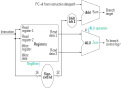
\includegraphics[scale=0.8]{imgBook/MIPS_datapath_branch_F9.pdf}
    \end{textblock}
    \begin{textblock}{100}(8,15)
    La instrucción salto por igualdad es de la forma:\\
    \hspace{0.28cm} \verb|beq $t1, $t2, offset|\\
    \bigskip
    \small
    \uncover<2->{\textcolor{verdeuca}{Toma tres operandos, dos registros\\ que serán comparados por igualdad\\ y un offset de 16 bits utilizado para\\ calcular la dirección destino del salto.}\\}
    \bigskip
    \normalsize
    \uncover<3->{\textbf{Observaciones}}\\
    \begin{itemize}
    \item<3-> El calculo de la dirección se realiza\\ sobre el valor del PC + 4.
    \item<4-> El offset se multiplica por 4 ya que\\ las instrucciones son de 32 bits.
    \end{itemize}
    \uncover<5->{\small \textcolor{gray}{La ALU provee una señal que indica si el\\ resultado de la operación es cero.}}
    \end{textblock}
    % The jump instruction operates by replacing the lower 28 bits of the PC with the
    % lower 26 bits of the instruction shifted left by 2 bits. Simply concatenating 00 to the
    % jump offset accomplishes this shift, as described in Chapter 2.
\end{frame}

\begin{frame}[t,fragile]
    \frametitle{Construyendo un Datapath: Observaciones}
    Examinamos los distintos caminos posibles para resolver las diferentes instrucciones.\\
    \uncover<2->{\textcolor{verdeuca}{Ahora buscamos combinar todo en un solo \emph{datapath} y agregar las señales de control necesarias.}\\}
    \bigskip
    \uncover<3->{Esta solución permitirá \textcolor{naranjauca}{\textbf{ejecutar una instrucción por ciclo de reloj}.}\\}
    \uncover<4->{Esto significa que \textcolor{rojo}{\textbf{ningún recurso puede ser usado más de una vez por instrucción}.}\\}
    \bigskip
    \uncover<5->{De ser necesario, los recursos deben ser:\\}
    \begin{itemize}
     \item<5-> \textbf{Duplicados}: Como sucede con los sumadores para calcular direcciones y operaciones.
     \item<6-> \textbf{Compartidos}: Como sucede con el banco de registros y sus puertos.
     \item<7-> \textbf{Divididos}: Como sucede con las memorias de datos y código.
    \end{itemize}
    \begin{center}
     \uncover<7->{\textcolor{verdeuca}{Es fundamental como parte del diseño de un \emph{datapath} entender\\
     como las instrucciones utilizarán los componentes en cada ciclo.}}
    \end{center}
\end{frame}

\begin{frame}[t,fragile]
    \frametitle{Construyendo un Datapath}
    Colocando todos los componentes juntos para resolver las instrucciones \emph{R-format}
    \begin{center}
    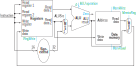
\includegraphics[scale=0.9]{imgBook/MIPS_datapath_memory_F10.pdf}
    \end{center}
\end{frame}

\begin{frame}[t,fragile]
    \frametitle{Simple Datapath}
    \begin{center}
    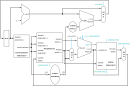
\includegraphics[scale=0.85]{imgBook/MIPS_simple_datapath_F11.pdf}
    \end{center}
\end{frame}

\begin{frame}[t,fragile]
    \frametitle{Control de la ALU}
    \begin{textblock}{80}(90,12)
    
\includegraphics[scale=1]{imgBook/MIPS_alu_signals.pdf}
    \end{textblock}
    \begin{textblock}{80}(60,47)
    \uncover<3->{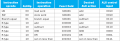
\includegraphics[scale=0.8]{imgBook/MIPS_alu_control_inputs_C4F12.pdf}}
    \end{textblock}
    \begin{textblock}{140}(10,12)
    \small
    Supongamos una ALU limitada a 5 operaciones.\\
    Dependiendo del tipo de instrucción, la ALU deberá\\ realizar diferentes operaciones.\\
    \bigskip
    \uncover<2->{
    Para simplificar el control podemos identificar la\\
    operación a realizar utilizando los bits de función\\
    y 2 bits de control para seleccionar la operación.\\
    }
    \bigskip
    \uncover<3->{
    Los bits de control (\texttt{ALUOp}) indican:
    \begin{itemize}
     \item[\texttt{00}] Operación ADD.\\ Para \emph{load/store}.
     \item[\texttt{01}] Operación SUB.\\ Para \emph{branch equal}.
     \item[\texttt{10}] Determinado por los bits\\ de función. Para \emph{R-type}
    \end{itemize}
    }
    \end{textblock}
\end{frame}

\begin{frame}[t,fragile]
    \frametitle{Control de la ALU}
    Considerando todos los bits obtenemos la siguiente tabla de verdad.
    \begin{center}
    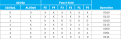
\includegraphics[scale=1]{imgBook/MIPS_alu_truth_table_C4F13.pdf}
    \end{center}
    \small
    \pause
    Observar que la tabla contiene \texttt{x} (don't-care) bits.\\
    Como \texttt{ALUOp} no puede valer \texttt{11}, se considera \texttt{x1} y \texttt{1x} en la tabla de verdad.\\
    Los bits de F5 y F4 siempre son siempre \texttt{10} para los últimos 5 casos, por lo tanto se ignoran.\\
    \bigskip
    \normalsize
    \textcolor{verdeuca}{Esta tabla ahora puede ser optimizada al momento de ser convertida en compuertas.}
\end{frame}

\begin{frame}[t,fragile]
    \frametitle{Formatos de instrucción}
    \vspace{-0.2cm}
    \begin{center}
    
\includegraphics[scale=1]{imgBook/MIPS_instruction_class_C4F14.pdf}
    \end{center}
    \small
    \pause
    \begin{itemize}
    \setlength\itemsep{-0.1cm}
    \item Los bits 31:26 refieren al Opcode (\texttt{Op[5:0]}). Los registros a leer \texttt{rs} (bits 25:21) y \texttt{rt} (bits 20:16).
    \item El registro base para \emph{load}/\emph{store} es \texttt{rs} en bits 25:21.
    \item El offset de 16-bit para \emph{branch equal} y \emph{load}/\emph{store} se toma de los bits 15:0.
    \item El registro destino puede ser \texttt{rt} para \emph{load} y \texttt{rd} para instrucciones \emph{R-type}.
    \end{itemize}
    \textcolor{verdeuca}{Vamos a requerir un multiplexor adicional para seleccionar el registro donde escribir.}
\end{frame}

\begin{frame}[plain,t,fragile]
    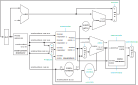
\includegraphics[scale=1]{imgBook/MIPS_simple_datapath_multiplex_F15.pdf}
    \begin{textblock}{80}(8,78)
    \textcolor{naranjauca}{\Large MIPS Simple Datapath}
    \end{textblock}
\end{frame}

\begin{frame}[plain,t,fragile]
    \begin{textblock}{80}(28,2)
    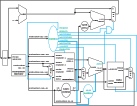
\includegraphics[scale=0.8]{imgBook/MIPS_simple_datapath_control_F17.pdf}
    \end{textblock}
    \begin{textblock}{80}(8,78)
    \textcolor{naranjauca}{\Large MIPS Simple Datapath\\ \normalsize Con lineas de control}
    \end{textblock}
\end{frame}

\begin{frame}[t,fragile]
    \frametitle{Unidad de control}
    La unidad de control funciona como una máquina de estados, sin embargo,\\
    en este caso cada instrucción que se realiza \textbf{en un solo ciclo}.\\
    \uncover<2->{
    \textcolor{verdeuca}{Por lo tanto la codificación de cada instrucción corresponde a un conjunto de señales de control.}\\
    \begin{center}
    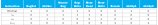
\includegraphics[scale=0.8]{imgBook/MIPS_control_lines_by_opcode_C4F18.pdf}
    \end{center}
    }
    \small
    \begin{enumerate}
     \item<3-> Instrucciones \emph{R-format}. Los registros \texttt{rs} y \texttt{rt} se utilizan como fuente, y \texttt{rd} como destino (\texttt{RegDst=1}). Los bits de \texttt{ALUOp} seleccionan \texttt{10} para usar los bits de función.
     \item<4-> Los bits de \texttt{ALUOp=00} para sumar con la ALU. Las señales para leer de memoria y escribir en \texttt{rt} (\texttt{RegDst=0}).
     \item<5-> Los bits de \texttt{ALUOp=00} para sumar con la ALU. Las señales para escribir en memoria y leer de \texttt{rt}.
     \item<6-> Los bits de \texttt{ALUOp=01} para restar con la ALU. La señal de \texttt{branch=1} para saltar condicionalmente. 
    \end{enumerate}
\end{frame}

\begin{frame}[t,fragile]
    \begin{textblock}{80}(28,2)
    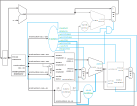
\includegraphics[scale=0.8]{imgBook/MIPS_simple_datapath_R-type_F19.pdf}
    \end{textblock}
    \begin{textblock}{80}(8,78)
    \textcolor{naranjauca}{\Large MIPS Simple Datapath\\ \normalsize Control para instrucciones R-type}
    \end{textblock}
\end{frame}

\begin{frame}[t,fragile]
    \begin{textblock}{80}(28,2)
    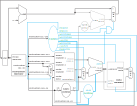
\includegraphics[scale=0.8]{imgBook/MIPS_simple_datapath_load_F20.pdf}
    \end{textblock}
    \begin{textblock}{80}(8,78)
    \textcolor{naranjauca}{\Large MIPS Simple Datapath\\ \normalsize Control para instrucción \emph{load}}
    \end{textblock}
\end{frame}

\begin{frame}[t,fragile]
    \begin{textblock}{80}(28,2)
    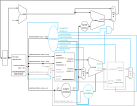
\includegraphics[scale=0.8]{imgBook/MIPS_simple_datapath_branch_F21.pdf}
    \end{textblock}
    \begin{textblock}{80}(8,78)
    \textcolor{naranjauca}{\Large MIPS Simple Datapath\\ \normalsize Control para instrucción \emph{branch equal}}
    \end{textblock}
\end{frame}

\begin{frame}[t,fragile]
    \frametitle{Unidad de control}
    Luego queda construir los estados de la unidad de control.
    \begin{center}
    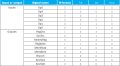
\includegraphics[scale=0.9]{imgBook/MIPS_control_unit_function_C4F22.pdf}
    \end{center}
    \vspace{-0.3cm}
    La tabla considera como entradas el opcode y salidas las señales de control de nuestro \emph{datapath}.
\end{frame}

\begin{frame}[t,fragile]
    \frametitle{Instrucción \emph{jump}}
    Nos resta agregar en nuestro \emph{datapath} la instrucción para saltos incondicionales.
    \begin{center}
    
\includegraphics[scale=0.9]{imgBook/MIPS_jump_instruction_C4F23.pdf}
    \end{center}
    \pause
    En MIPS está instrucción calcula la dirección de la siguiente forma:
    \begin{itemize}
     \item \textcolor{verdeuca}{Se toma un inmediato de 26 bits de la instrucción.}
     \item \textcolor{verdeuca}{Los dos bits menos significativos se los completan con \texttt{0}.}
     \item \textcolor{verdeuca}{Los cuatro bits más significativos corresponden al valor del \texttt{PC+4}.}
    \end{itemize}
    Con esto tenemos un valor de 32 bits para usar como dirección destino.\\
    \pause
    \bigskip
    Al \emph{datapath} debemos agregar:
    \begin{itemize}
     \item \textcolor{verdeuca}{Tomar los 26 bits como parte de la decodificación de la instrucción.}
     \item \textcolor{verdeuca}{Un componente que realice el shift de 2 bits.}
     \item \textcolor{verdeuca}{Un componente que combine los bits entre el \texttt{PC+4} y el valor calculado.}
    \end{itemize}
\end{frame}

\begin{frame}[t,fragile]
    \begin{textblock}{80}(28,2)
    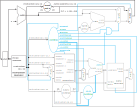
\includegraphics[scale=0.8]{imgBook/MIPS_simple_datapath_jmp_F24.pdf}
    \end{textblock}
    \begin{textblock}{80}(8,78)
    \textcolor{naranjauca}{\Large MIPS Simple Datapath\\ \normalsize Control para instrucción \emph{jump}}
    \end{textblock}
\end{frame}

\begin{frame}[t,fragile]
    \frametitle{¿Podemos hacer algo mejor?}
    Si bien el diseño en un solo ciclo es funciona, no es utilizado ya que es \textbf{ineficiente}.\\
    \bigskip
    \pause
    \textcolor{verdeuca}{Notar que cada instrucción debe demorar \textbf{lo mismo} en un diseño \emph{single-cycle}.}\\
    \textcolor{rojo}{Esto implica que todas van a demorar lo mismo que \textbf{el camino más costoso}.}\\
    Este camino es una instrucción de \emph{load}, que utiliza \textbf{todas las unidades funcionales}.\\
    \pause
    \bigskip
    \textcolor{gray}{La penalidad de un diseño con \textbf{el tiempo de reloj fijo} es muy alta y solo puede ser considerada para conjuntos de instrucciones pequeños.}\\
    \bigskip
    \pause
    \textcolor{gray}{Si nuestro conjunto de instrucciones es complejo, o incluye instrucciones de punto flotante, \textbf{debemos asumir el peor retardo para todas las instrucciones},
    cualquier esfuerzo por reducir el retardo para el caso común no va a mejorar el peor caso.}\\
    \bigskip
    Un diseño \emph{single-cycle} no respeta el objetivo de hacer el caso común lo más rápido posible.
\end{frame}

% % % % % % % % % % % % % % % % % % % % PIPELINE

\begin{frame}[t,fragile]
    \frametitle{Segmentación (\emph{Pipelining})}
    \textcolor{naranjauca}{\emph{Pipelining} es una técnica de implementación de procesadores en la cual \textbf{se superpone la ejecución} de múltiples instrucciones.}
    \uncover<2->{La idea es \textbf{dividir el trabajo} en etapas (\emph{stages}), donde en cada etapa se puede ejecutar una sola instrucción a la vez.}\\
    \vspace{0.2cm}
    \uncover<3->{\textcolor{verdeuca}{Veamos un ejemplo con una fabrica de autos.}}\\
    \begin{textblock}{80}(10 ,34) \only<3>{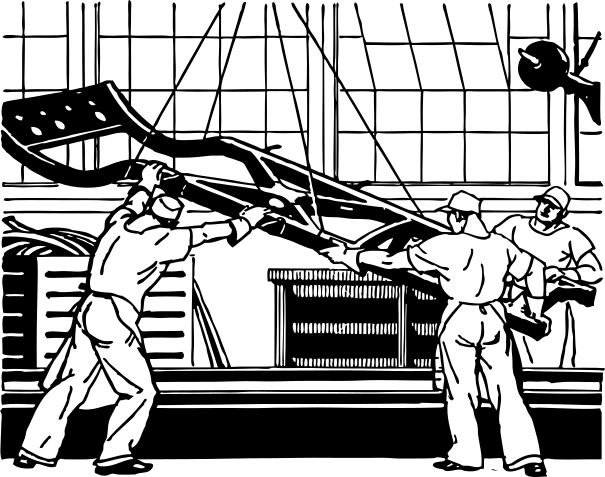
\includegraphics[scale=0.2]{img/line_1_johnny_automatic_frame_goes_on_the_assembly_line.pdf}} \end{textblock}
    \begin{textblock}{80}(45 ,34) \only<4>{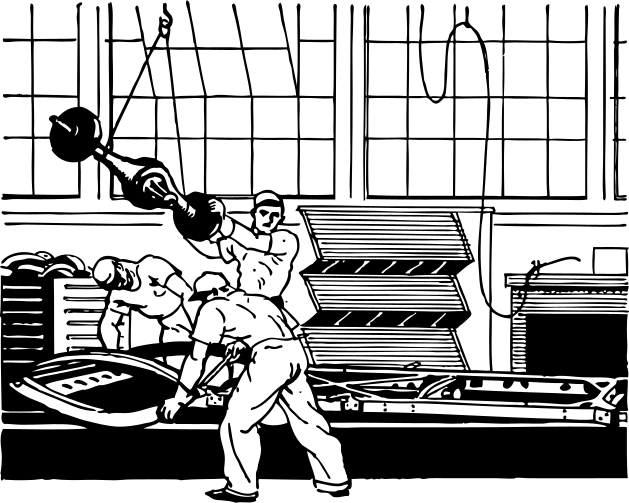
\includegraphics[scale=0.2]{img/line_2_johnny_automatic_putting_the_axle_on_the_chasis.pdf}} \end{textblock}
    \begin{textblock}{80}(80 ,34) \only<5>{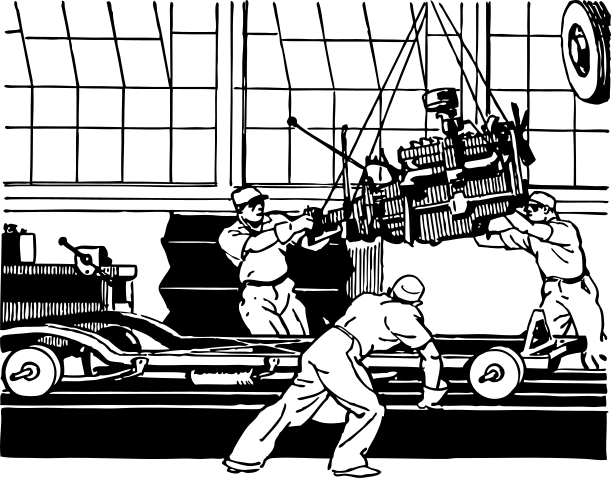
\includegraphics[scale=0.2]{img/line_3_johnny_automatic_here_comes_the_engine.pdf}} \end{textblock}
    \begin{textblock}{80}(115,34) \only<6>{\includegraphics[scale=0.2]{img/line_4_johnny_automatic_fastening_the_wheels.pdf}} \end{textblock}
    \begin{textblock}{80}(10 ,62) \only<7>{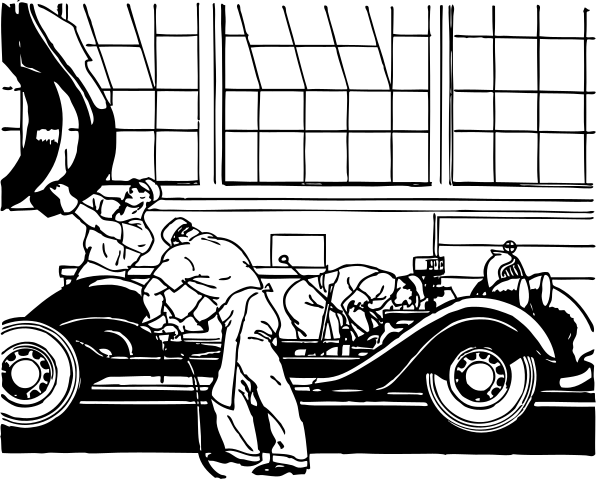
\includegraphics[scale=0.2]{img/line_5_johnny_automatic_bolting_on_fenders_and_running_boards.pdf}} \end{textblock}
    \begin{textblock}{80}(45 ,62) \only<8>{\includegraphics[scale=0.2]{img/line_6_johnny_automatic_lowering_the_body.pdf}} \end{textblock}
    \begin{textblock}{80}(80 ,62) \only<9>{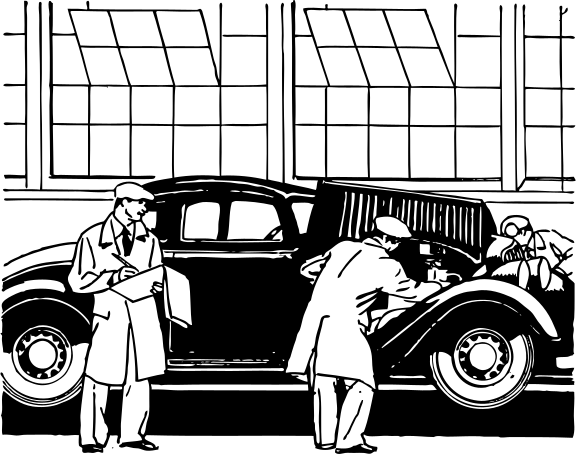
\includegraphics[scale=0.2]{img/line_7_johnny_automatic_final_inspection.pdf}} \end{textblock}
    \begin{textblock}{80}(115,62) \only<10>{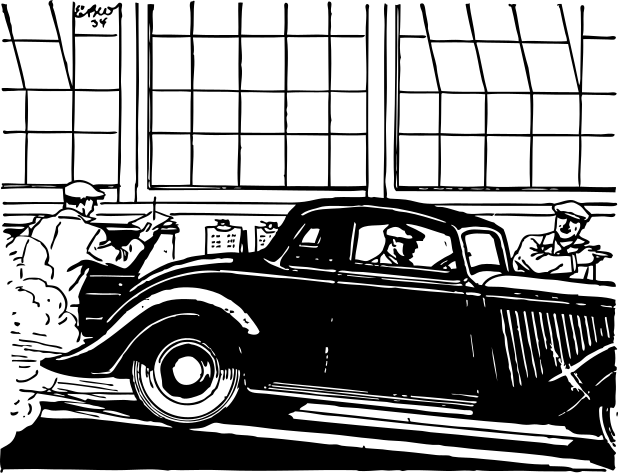
\includegraphics[scale=0.2]{img/line_8_johnny_automatic_rolling_off_the_assembly_line.pdf}} \end{textblock}
    \begin{textblock}{80}(10 ,34) \only<11>{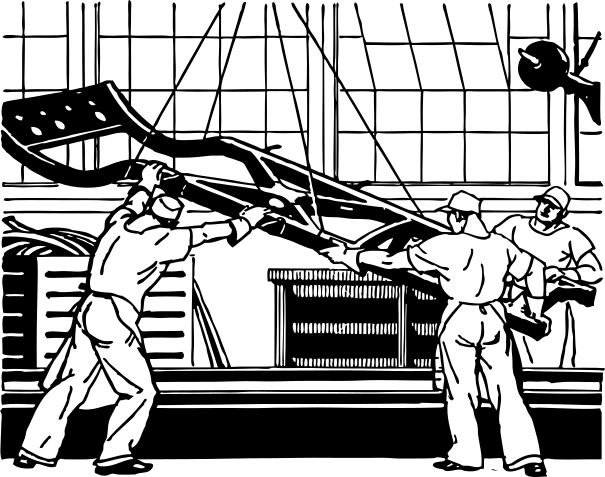
\includegraphics[scale=0.2]{img/line_1_johnny_automatic_frame_goes_on_the_assembly_line.pdf}} \end{textblock}
    \begin{textblock}{80}(45 ,34) \only<11>{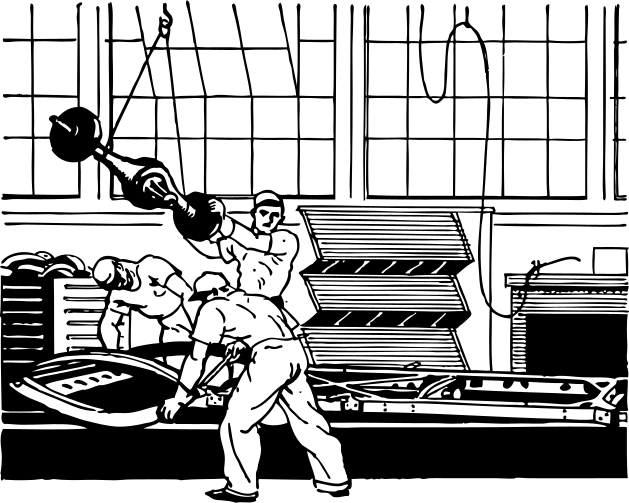
\includegraphics[scale=0.2]{img/line_2_johnny_automatic_putting_the_axle_on_the_chasis.pdf}} \end{textblock}
    \begin{textblock}{80}(80 ,34) \only<11>{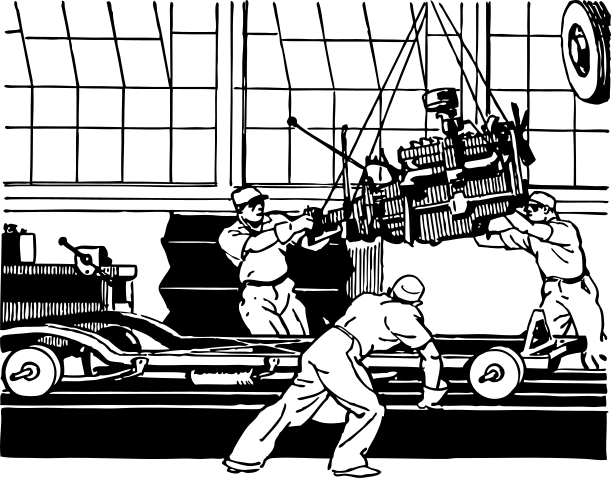
\includegraphics[scale=0.2]{img/line_3_johnny_automatic_here_comes_the_engine.pdf}} \end{textblock}
    \begin{textblock}{80}(115,34) \only<11>{\includegraphics[scale=0.2]{img/line_4_johnny_automatic_fastening_the_wheels.pdf}} \end{textblock}
    \begin{textblock}{80}(10 ,62) \only<11>{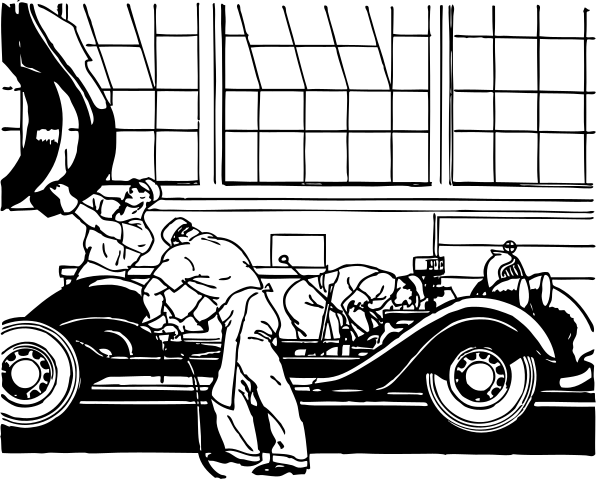
\includegraphics[scale=0.2]{img/line_5_johnny_automatic_bolting_on_fenders_and_running_boards.pdf}} \end{textblock}
    \begin{textblock}{80}(45 ,62) \only<11>{\includegraphics[scale=0.2]{img/line_6_johnny_automatic_lowering_the_body.pdf}} \end{textblock}
    \begin{textblock}{80}(80 ,62) \only<11>{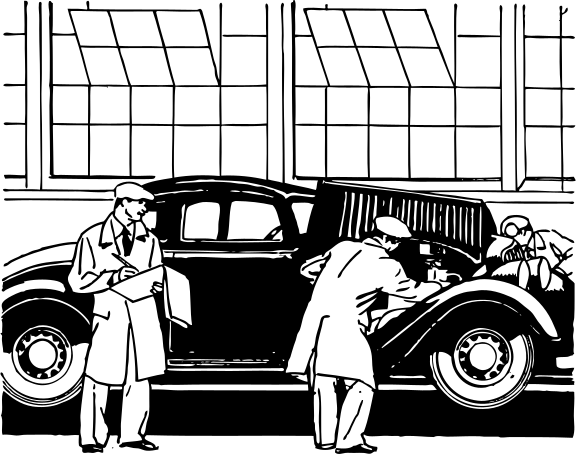
\includegraphics[scale=0.2]{img/line_7_johnny_automatic_final_inspection.pdf}} \end{textblock}
    \begin{textblock}{80}(115,62) \only<11>{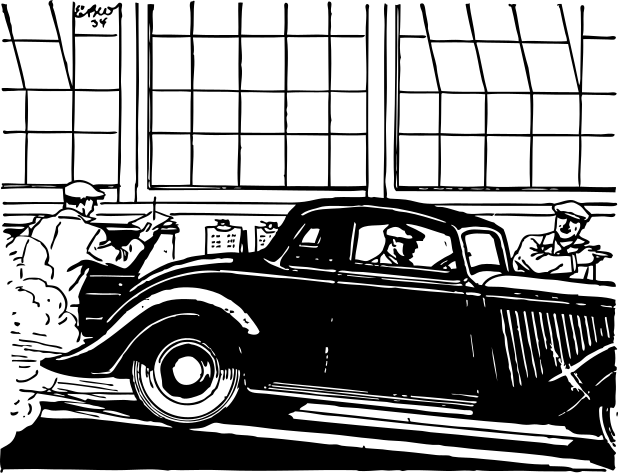
\includegraphics[scale=0.2]{img/line_8_johnny_automatic_rolling_off_the_assembly_line.pdf}} \end{textblock}
\end{frame}

\begin{frame}[t,fragile]
    \frametitle{Segmentación (\emph{Pipelining})}
    Usando la misma idea aplicada a las instrucciones de un procesador podemos construir un \emph{pipeline} o un procesador segmentado.\\
    \bigskip
    \pause
    Un diseño posible para MIPS es el \textbf{\emph{pipeline} de cinco etapas}.
    \bigskip
    \begin{enumerate}
    \setlength\itemsep{0.2cm}
     \item Leer la instrucción de memoria (\emph{Fetch}).
     \item Leer registros mientras se decodifica la instrucción.
     \item Ejecutar la operación o calcular una dirección.
     \item Acceder a los operandos en memoria.
     \item Escribir el resultado en un registro.
    \end{enumerate}
\end{frame}

% To make this discussion concrete, let’s create a pipeline. 
% In this example, and in the rest of this chapter, we limit our attention to eight instructions: 
% load word (lw), store word (sw), add (add), subtract (sub), AND (and), OR (or), set less than (slt), and branch on equal (beq).

\begin{frame}[t,fragile]
    \frametitle{\emph{Single-Cycle} vs \emph{Pipelined}}
    \begin{textblock}{45}(110,8)
    \small
    \uncover<2->{
    \textcolor{gray}{Ejemplo:}\\
    \vspace{0.1cm}
    \hspace{0.2cm} 200 ps para accesos a memoria.\\
    \hspace{0.2cm} 200 ps para operaciones (ALU).\\
    \hspace{0.2cm} 100 ps para acceder a registros.\\
    \vspace{0.2cm}
    \textcolor{verdeuca}{El ciclo se debe acomodar al tiempo de la instrucción más lenta.}
    }
    \end{textblock}
    \begin{textblock}{45}(110,60)
    \small
    \uncover<4->{
    \textcolor{verdeuca}{Cada etapa se debe diseñar para el peor caso de 200 ps, incluso si algunas etapas pueden demorar menos.}
    }
    \end{textblock}
    \small
    \uncover<1->{
    \textcolor{verdeuca}{Implementación \emph{single-cycle}:} Cada instrucción demora un ciclo de reloj.\\   
    \vspace{0.2cm}
    \includegraphics[scale=0.75]{imgBook/single_cycle_nonpipelined_F27-layer1.pdf}\\
    }
    \uncover<3->{
    \textcolor{verdeuca}{Implementación \emph{pipelined}:} Cada etapa esta acotada al tiempo de la etapa más costosa.\\
    \vspace{0.2cm}
    \includegraphics[scale=0.75]{imgBook/single_cycle_nonpipelined_F27-layer2.pdf}
    }
\end{frame}

\begin{frame}[t,fragile]
    \frametitle{Diseño de un ISA para una implementación Segmentada}
    \small
    El diseño de un ISA debe respetar \textbf{máximas} que faciliten su implementación segmentada.\\
    \textcolor{verdeuca}{En particular, MIPS las respeta.}
    \begin{itemize}
    \item<2-> \textcolor{naranjauca}{\textbf{Todas las instrucciones de la misma longitud.}}\\
    Esto facilita la decodificación y simplifica la etapa de \emph{fetch}.
    \textcolor{gray}{En un \texttt{x86} donde el tamaño de las instrucciones es variable y está tarea es mucho más desafiante.}
    \item<3-> \textcolor{naranjauca}{\textbf{Tener pocos formatos de instrucción.}}\\
    Con campos de parámetros en los mismos lugares para cada instrucción.
    Está regularidad permite acceder al banco de registros al mismo tiempo que se determina la operación de la instrucción.
    \textcolor{gray}{Si no fueran regulares deberíamos generar más etapas del \emph{pipeline} para decodificar y acceder a los registros.}
    \item<4-> \textcolor{naranjauca}{\textbf{Los operandos de memoria solo aparecen para escrituras y lecturas a memoria.}}\\
    Podemos usar la etapa de ejecución para calcular la dirección de memoria y luego acceder a la memoria en la siguiente etapa.
    \textcolor{gray}{Si pudiéramos operar con operandos en memoria, como en el x86, se deberían crear más etapas.}
    \item<5-> \textcolor{naranjauca}{\textbf{Los operandos deben estar alineados a memoria.}}\\
    Nos permite asegurarnos que se requiere una sola transferencia entre el procesador y la memoria.
    \end{itemize}
\end{frame}

\begin{frame}[t,fragile]
    \frametitle{Pipeline Hazards}
    \small
    Existen situaciones en las que la próxima instrucción \textbf{no puede ser ejecutada} en el siguiente ciclo.\\
    \textcolor{verdeuca}{Estos eventos se denominan \textbf{\emph{hazards}}.}\\
    \bigskip
    \pause
    \textcolor{naranjauca}{\textbf{Structural Hazard}}\\
    \vspace{0.2cm}
    Sucede cuando el hardware no puede soportar una determinada combinación de instrucciones en el mismo ciclo.
    \textcolor{gray}{Por ejemplo, si la memoria de instrucciones y datos fuera la misma, no se podría en el mismo ciclo hacer una escritura a memoria y una lectura de la nueva instrucción.}\\
    \vspace{0.2cm}
    \pause
    \textcolor{naranjauca}{\textbf{Data Hazard}}\\
    \vspace{0.2cm}
    Ocurre cuando el \emph{pipeline} debe ser detenido (\emph{stall}) porque se requiere que la instrucción anterior esté completa.
    \textcolor{gray}{Por ejemplo, las instrucciones \texttt{add \$s0, \$t0, \$t1}; \texttt{sub \$t2, \$s0, \$t3}; dependen que \texttt{\$s0} tenga el valor de la suma antes de ejecutar la resta.}
    Las instrucciones dependen entre sí.\\
    \vspace{0.2cm}
    \pause
    \textcolor{naranjauca}{\textbf{Control Hazard}}\\
    \vspace{0.2cm}
    Aparece cuando se debe tomar una decisión basada en el resultado de una operación.
    \textcolor{gray}{Luego del \emph{fetch} debemos calcular cual es la próxima instrucción. Pero si esta es un salto condicional, debemos esperar a que la misma se ejecute, esperando el calculo del nuevo PC.}
\end{frame}

\begin{frame}[t,fragile]
    \frametitle{Data Hazard - \emph{Forwarding}}
    \begin{textblock}{60}(8,12)
    \small
    La solución está basada en la observación:\\
    \textcolor{verdeuca}{\textbf{no es necesario esperar a que se termine\\
    la instrucción para resolver el problema.}}\\
    \bigskip
    \uncover<2->{
    \textcolor{gray}{Por ejemplo, para la secuencia de suma y resta, podemos, una vez terminada la suma en la ALU, usar ese resultado en la resta.}\\
    }
    \bigskip
    \uncover<3->{
    \textbf{\emph{Forwarding}} o \textbf{\emph{Bypassing}}\\
    Hardware adicional para identificar\\
    el dato faltante desde los recursos\\
    internos y proveerlo para usarlo en\\
    la próxima instrucción.
    }
    \end{textblock}
    \begin{textblock}{10}(65,12)
    \includegraphics[scale=0.75]{imgBook/instruction_pipeline_representation_F28_F29_F30-layer1.pdf}\\
    \uncover<3->{\includegraphics[scale=0.75]{imgBook/instruction_pipeline_representation_F28_F29_F30-layer2.pdf}}
    \end{textblock}
\end{frame}

\begin{frame}[t,fragile]
    \frametitle{Data Hazard - \emph{Forwarding}}
    \begin{textblock}{50}(8,12)
    \small
    No siempre es posible disponer del dato para la próxima instrucción.\\
    \bigskip
    \uncover<2->{\textcolor{gray}{Por ejemplo,}\\}
    \begin{itemize}
    \item<2-> \textcolor{gray}{Si la primer instrucción es un \texttt{load} al registro \texttt{\$s0}.}
    \item<3-> \textcolor{gray}{El dato para operar con la siguiente instrucción recién lo vamos a obtener luego de la etapa 4 donde leemos a memoria.}
    \item<4-> \textcolor{gray}{Este dato lo vamos a tener muy tarde para llegar a hacer un \emph{forwarding}.}
    \end{itemize}
    \end{textblock}
    \begin{textblock}{85}(65,55)
    \small
    \uncover<5->{
    En este caso estamos obligados a agregar un \emph{stall} en el \emph{pipeline}.
    \textcolor{verdeuca}{Usualmente la etapa sin operación se denomina \emph{bubble}.}\\
    }
    \bigskip
    \uncover<6->{
    Hardware especial permite detectar estos casos y generar los \emph{bubble} artificialmente.
    \textcolor{verdeuca}{Incluso podemos reordenar el código para reducir la necesidad de tener \emph{pipeline} \emph{stalls}.}
    }
    \end{textblock}
    \begin{textblock}{10}(63,12)
    \uncover<2->{\includegraphics[scale=0.75]{imgBook/instruction_pipeline_representation_F28_F29_F30-layer3.pdf}}
    \end{textblock}
\end{frame}

\begin{frame}[t,fragile]
    \frametitle{Control Hazard - \emph{Branch Prediction}}
    \begin{textblock}{50}(10,12)
    \small
    La dirección del salto recién será resuelta en la segunda etapa.\\
    \bigskip
    \textcolor{verdeuca}{Por lo tanto vamos a tener que esperar un ciclo más antes de conocer la nueva instrucción.}\\
    \bigskip
    Esto obliga a agregar un ciclo \emph{stall}.\\
    \end{textblock}
    \begin{textblock}{140}(10,50)
    \small
    \uncover<2->{
    \textcolor{naranjauca}{Las instrucciones de salto representan en promedio un 17\%,\\
    por lo tanto para todas estas instrucciones \textbf{desperdiciariamos un ciclo}.}}
    \uncover<3->{\textbf{¿Podemos hacer algo mejor?}\\}
    \bigskip
    \uncover<4->{\textcolor{v}{\textbf{¡Predecir!}}\\}
    \bigskip
    \uncover<4->{La idea es simple, podemos asumir que los saltos nunca se toman, y si se llegan a tomar, pagamos el costo de un \emph{stall}.
    \textcolor{gray}{La instrucción se ejecutará especulativamente, sin escribir nada y luego se confirma.}}
    \end{textblock}
    \begin{textblock}{10}(63,12)
    \includegraphics[scale=0.75]{imgBook/instruction_pipeline_branch_F31_F32-layer1.pdf}
    \end{textblock}
\end{frame}

\begin{frame}[t,fragile]
    \frametitle{Control Hazard - \emph{Branch Prediction}}
    \begin{textblock}{45}(10,14)
    \small
    Procesadores modernos, utilizan sofisticados predictores de saltos.\\
    \bigskip
    \uncover<2->{
    \textcolor{verdeuca}{La predicción dinámica utiliza información historica del programa
    y cambia su predicción durante la vida de este.}\\
    }
    \bigskip
    \uncover<4->{
    \textcolor{gray}{La precisión de los predictores de saltos es mayor al 90\%}\\
    }
    \bigskip
    \uncover<5->{
    Otra técnica es \emph{delayed branch}, donde se demora la decisión de tomar el salto, agregando una instrucción luego del salto que se ejecuta siempre.
    }
    \end{textblock}
    \begin{textblock}{50}(63,12) \small
    \uncover<3->{
    \hspace{1.2cm}\textbf{\textcolor{naranjauca}{Branch Not Taken}}
    \includegraphics[scale=0.75]{imgBook/instruction_pipeline_branch_F31_F32-layer2.pdf}\\
    \hspace{1.2cm}\textbf{\textcolor{naranjauca}{Branch Taken}}
    \includegraphics[scale=0.75]{imgBook/instruction_pipeline_branch_F31_F32-layer3.pdf}
    }
    \end{textblock}
\end{frame}

\begin{frame}[t,fragile]
    \frametitle{Datapath Segmentado}
    \begin{textblock}{70}(6,12)
    \small
    Sobre el datapath single-cycle\\
    identificamos las etapas\\
    del \emph{pipeline}.\\
    \vspace{0.2cm}
    \uncover<2->{
    \textcolor{verdeuca}{En un \emph{pipeline} de cinco\\
    etapas, 5 instrucciones\\
    serán ejecutadas al\\
    mismo tiempo.}\\
    }
    \vspace{0.2cm}
    \uncover<3->{
    Debemos separar\\
    el datapath en cinco etapas.
    }
    \begin{enumerate}
    \item<3-> \textcolor{naranjauca}{\textbf{IF}}: Instruction Fetch
    \item<3-> \textcolor{naranjauca}{\textbf{ID}}: Instruction Decode and register file read
    \item<3-> \textcolor{naranjauca}{\textbf{EX}}: EXecution or address calculation
    \item<3-> \textcolor{naranjauca}{\textbf{MEM}}: Data MEMory access
    \item<3-> \textcolor{naranjauca}{\textbf{WB}}: Write Back
    \end{enumerate}
    \end{textblock}
    \begin{textblock}{140}(41,3)
    \includegraphics[scale=0.8]{imgBook/MIPS_simple_datapath_single_cycle_steps_F33.pdf}
    \end{textblock}
\end{frame}

\begin{frame}[t,fragile]
    \frametitle{Datapath Segmentado}
    \begin{textblock}{70}(6,29)
    \small
    Los datos en el datapath\\
    se mueven de \textbf{izquierda\\
    a derecha} siguiendo las\\
    etapas del \emph{pipeline}.\\
    \bigskip
    \uncover<2->{Con dos excepciones:}
    \begin{itemize}
     \item<2-> \textcolor{naranjauca}{\textbf{En la etapa de \emph{write-back}}}\\
     Se escribe el resultado en el banco\\
     de registros, a la mitad del \emph{pipeline}.
     \item<3-> \textcolor{naranjauca}{\textbf{En la selección del próximo PC}}\\
     Eligiendo entre incrementar el PC y la\\
     dirección de salto en la etapa de memoria.
    \end{itemize}
    \end{textblock}
    \begin{textblock}{140}(41,3)
    \includegraphics[scale=0.8]{imgBook/MIPS_simple_datapath_single_cycle_steps_F33.pdf}
    \end{textblock}
\end{frame}

\begin{frame}[t,fragile]
    \frametitle{Datapath Segmentado}
    \begin{textblock}{50}(10,12)
    \small
    Una forma de ver la ejecución segmentada de instrucciones es pretender que existe \textbf{un datapath exclusivo para cada instrucción}.\\
    \uncover<2->{\textcolor{verdeuca}{Luego, agrupar esos datapath en el tiempo y así ver sus relaciones.}\\}
    \bigskip
    \uncover<3->{
    \textcolor{naranjauca}{Para compartir el datapath debemos agregar registros que \textbf{mantengan la información} a medida que la instrucción recorre el \emph{pipeline}.}\\
    }
    \bigskip
    \uncover<4->{
    \textcolor{gray}{Cada una de las etapas es utilizada por solo una instrucción por ciclo.\\
    \textbf{Entonces podemos compartirlas en los cuatro ciclos restantes}.}
    }
    \end{textblock}
    \begin{textblock}{140}(66,15)
    \uncover<2->{\includegraphics[scale=0.8]{imgBook/single_cycle_as_pipeline_steps_F34.pdf}}
    \end{textblock}
\end{frame}

\begin{frame}[t,fragile]
    \frametitle{Datapath Segmentado}
    \begin{textblock}{140}(5,3)
    \includegraphics[scale=0.93]{imgBook/MIPS_pipeline_datapath_F35_F46.pdf}
    \end{textblock}
\end{frame}

\begin{frame}[t,fragile]
    \frametitle{Datapath Segmentado}
    \vspace{0.5cm}
    En el diseño se observa:\\
    \bigskip
    \begin{itemize}
    \setlength\itemsep{0.2cm}
    \item<2-> Las instrucciones \textbf{avanzan} de etapa por cada ciclo de reloj.
    \item<3-> Se identifican un \textbf{conjunto de registros} para cada par de etapas.\\
    \textcolor{gray}{Estos se nombran como las dos etapas que los comparten.}
    \item<4-> No existe un registro para la \textbf{última etapa}, siempre escribe.
    \item<5-> Todas las instrucciones \textbf{deben modificar} el estado del procesador,\\
    banco de registros, memoria, PC.
    \end{itemize}
    \bigskip
    \uncover<6->{
    \textcolor{naranjauca}{Ahora resta entender que parte del datapath se \textbf{utiliza} en cada etapa.}\\
    \begin{center}
    \textcolor{verdeuca}{\textbf{Vamos a estudiar las instrucciones \texttt{lw} (\emph{load}) y \texttt{sw} (\emph{store})}}
    \end{center}
    }
\end{frame}

\begin{frame}[t,fragile]
    \frametitle{Datapath Segmentado - Load \large (Instruction fetch)}
    \begin{textblock}{140}(5,7) \includegraphics[scale=0.93]{imgBook/MIPS_pipeline_datapath_F35_F46-layer2.pdf} \end{textblock}
    \begin{textblock}{30}(5,70) \footnotesize
    Lectura de instrucción y actualización del PC.
    \end{textblock}
\end{frame}

\begin{frame}[t,fragile]
    \frametitle{Datapath Segmentado - Load \large (Instruction decode and register file read)}
    \begin{textblock}{140}(5,7) \includegraphics[scale=0.93]{imgBook/MIPS_pipeline_datapath_F35_F46-layer3.pdf} \end{textblock}
    \begin{textblock}{30}(5,70) \footnotesize
    Lectura de registro y extensión de signo de valor inmediato.
    \end{textblock}
\end{frame}

\begin{frame}[t,fragile]
    \frametitle{Datapath Segmentado \large (Address calculation)}
    \begin{textblock}{140}(5,7) \includegraphics[scale=0.93]{imgBook/MIPS_pipeline_datapath_F35_F46-layer4.pdf} \end{textblock}
    \begin{textblock}{30}(5,70) \footnotesize
    Calculo de la dirección destino.
    \end{textblock}
\end{frame}

\begin{frame}[t,fragile]
    \frametitle{Datapath Segmentado - Load \large (Memory access)}
    \begin{textblock}{140}(5,7) \includegraphics[scale=0.93]{imgBook/MIPS_pipeline_datapath_F35_F46-layer5.pdf} \end{textblock}
    \begin{textblock}{30}(5,70) \footnotesize
    Lectura de memoria.
    \end{textblock}
\end{frame}

\begin{frame}[t,fragile]
    \frametitle{Datapath Segmentado - Load \large (Write-back)}
    \begin{textblock}{140}(5,7) \includegraphics[scale=0.93]{imgBook/MIPS_pipeline_datapath_F35_F46-layer6.pdf} \end{textblock}
    \begin{textblock}{30}(5,70) \footnotesize
    Escritura en el banco de registros. 
    \uncover<2->{\textcolor{rojo}{\textbf{Pero ¿Dónde?}}}
    \end{textblock}
\end{frame}

\begin{frame}[t,fragile]
    \frametitle{Datapath Segmentado - Load \large (Write-back) $\rightarrow$ \textbf{Arreglado}}
    \begin{textblock}{140}(5,7) \includegraphics[scale=0.93]{imgBook/MIPS_pipeline_datapath_F35_F46-layer10.pdf} \end{textblock}
    \begin{textblock}{38}(5,70) \footnotesize
    Escritura en el banco de registros.
    \textcolor{verdeuca}{\textbf{Tenemos que llevar el estado de lugar donde escribir por todo el \emph{pipeline}}}.
    \end{textblock}
\end{frame}

\begin{frame}[t,fragile]
    \frametitle{Datapath Segmentado - Load}
    \begin{textblock}{140}(5,7) \includegraphics[scale=0.93]{imgBook/MIPS_pipeline_datapath_F35_F46-layer11.pdf} \end{textblock}
    \begin{textblock}{38}(5,70) \footnotesize
    Esta instrucción utiliza todas las unidades funcionales.
    \end{textblock}
\end{frame}

\begin{frame}[t,fragile]
    \frametitle{Datapath Segmentado - Store \large (Address calculation)}
    \begin{textblock}{140}(5,7) \includegraphics[scale=0.93]{imgBook/MIPS_pipeline_datapath_F35_F46-layer7.pdf} \end{textblock}
    \begin{textblock}{30}(5,70) \footnotesize
    Calculo de la dirección destino.
    \end{textblock}
\end{frame}

\begin{frame}[t,fragile]
    \frametitle{Datapath Segmentado - Store \large (Memory access)}
    \begin{textblock}{140}(5,7) \includegraphics[scale=0.93]{imgBook/MIPS_pipeline_datapath_F35_F46-layer8.pdf} \end{textblock}
    \begin{textblock}{30}(5,70) \footnotesize
    Escritura a memoria.
    \end{textblock}
\end{frame}

\begin{frame}[t,fragile]
    \frametitle{Datapath Segmentado - Store \large (Write-back)}
    \begin{textblock}{140}(5,7) \includegraphics[scale=0.93]{imgBook/MIPS_pipeline_datapath_F35_F46-layer9.pdf} \end{textblock}
    \begin{textblock}{30}(5,70) \footnotesize
    \textcolor{verdeuca}{La etapa de \emph{write back} se ejecuta pero \textbf{no realiza ninguna acción}.}
    \end{textblock}
\end{frame}

\begin{frame}[t,fragile]
    \frametitle{Representación gráfica de un \emph{pipeline}}
    \begin{textblock}{50}(105,12)
    \small
    Supongamos las siguientes instrucciones:
    \bigskip
    \footnotesize
    \texttt{lw \$10, 20(\$1)}\\
    \texttt{sub \$11, \$2, \$3}\\
    \texttt{add \$12, \$3, \$4}\\
    \texttt{lw \$13, 24(\$1)}\\
    \texttt{add \$14, \$5, \$6}\\
    \bigskip
    \small
    \uncover<2->{
    En el diagrama se puede \textbf{identificar que unidad está en uso} en cada ciclo de reloj para cada instrucción en ejecución.\\}
    \bigskip
    \uncover<3->{
    \textcolor{verdeuca}{Notar que el banco de registros se utiliza por dos instrucciones simultaneamente.}}
    \end{textblock}
    \begin{textblock}{140}(3,13)
\includegraphics[scale=0.7]{imgBook/pipeline_multicycle_diagram_F43.pdf}
    \end{textblock}
\end{frame}

\begin{frame}[t,fragile]
    \frametitle{Representación gráfica de un \emph{pipeline}}
    Otra forma de representar el \emph{pipeline} es indicando en que unidad se encuentra cada instrucción.
    \begin{center}
    \includegraphics[scale=0.8]{imgBook/pipeline_multicycle_diagram_blocks_F44.pdf}
    \end{center}
    \pause
    \textcolor{verdeuca}{En este caso se pierde que tarea está realizando cada unidad, o incluso si está en uso.}\\
    \vspace{0.2cm}
    \textcolor{naranjauca}{Veamos entonces el estado de todo el \emph{datapath} durante el quinto ciclo.}
\end{frame}

\begin{frame}[t,fragile]
    \frametitle{Datapath Segmentado - Quinto Ciclo}
    \begin{textblock}{140}(10,7) \includegraphics[scale=0.93]{imgBook/MIPS_pipeline_datapath_F35_F46-layer12.pdf} \end{textblock}
\end{frame}

\begin{frame}[t,fragile]
    \frametitle{Señales de control en un diseño segmentado}
    \small
    Usando las señales de control del diseño \emph{single-cycle} y el funcionamiento de la unidad de control.\\
    \vspace{0.2cm}
    \textcolor{verdeuca}{Vamos a asumir que el PC se escribe en todos los ciclos al igual que los registros de \emph{pipeline} (\texttt{IF\/ID}, \texttt{ID\/EX}, \texttt{EX\/MEM} y \texttt{MEM\/WB}),
    por lo tanto \textbf{no requieren una señal de control} para su escritura.\\}
    \vspace{0.2cm}
    \uncover<2->{
    Necesitamos especificar las señales de control.
    \textcolor{naranjauca}{Los valores de cada señal dependerán de la etapa del \emph{pipeline}, \textbf{ya que las señales de control dependen de cada componente activo en la etapa}.}\\
    }
    \vspace{0.2cm}
    \uncover<3->{Vamos a dividir las líneas de control en cinco grupos.\\}
    \begin{enumerate}
    \item<3-> \emph{Instruction fetch}: Las señales siempre están activas, no hay nada que hacer.
    \item<4-> \emph{Instruction decode\/register file read}: Las señales siempre están activas, no hay nada que hacer.
    \item<5-> \emph{Execution\/address calculation}: Las señales a configurar son \texttt{RegDst}, \texttt{ALUOp}, y \texttt{ALUSrc}.\\
    {\scriptsize \textcolor{gray}{Las señales seleccionan el registro resultado, la operación ALU, y una de las entradas de la ALU.}}
    %entre \texttt{Read} \texttt{data} \texttt{2} o \texttt{sign-extended} \texttt{immediate}.}}
    \item<6-> \emph{Memory access}: Las líneas de control configuradas en esta etapa son \texttt{Branch}, \texttt{MemRead} y \texttt{MemWrite}.
    {\scriptsize \textcolor{gray}{Las instrucciones \texttt{branch equal}, \texttt{load} y \texttt{store} establecen estas señales, respectivamente.}}
    \item<7-> \emph{Write-back}: Las dos líneas de control son \texttt{MemtoReg}, que decide entre enviar el resultado de la ALU o el valor de la memoria al banco de registros, y el registro destino.
    \end{enumerate}
\end{frame}

\begin{frame}[t,fragile]
    \frametitle{Datapath Segmentado - Indentificación de señales de control}
    \begin{textblock}{140}(10,3) \includegraphics[scale=0.84]{imgBook/MIPS_pipeline_datapath_F35_F46-layer13.pdf} \end{textblock}
\end{frame}

\begin{frame}[t,fragile]
\frametitle{Datapath Segmentado - Con señales de control}
    La forma más simple de implementar que cada instrucción traslade sus señales de control\\
    en el \emph{pipeline}, es \textcolor{naranjauca}{extendiendo los registros del \emph{pipeline} con las señales a mantener.}
    \begin{center}
    \includegraphics[scale=0.75]{imgBook/pipeline_control_stages_F50.pdf}
    \end{center}
\end{frame}

\begin{frame}[t,fragile]
    \begin{textblock}{140}(30,2) \includegraphics[scale=0.76]{imgBook/pipeline_datapath_control_F51.pdf} \end{textblock}
    \begin{textblock}{50}(10,70)
    {\Large \textcolor{naranjauca}{Datapath Segmentado\\ Con señales de control}}
    \end{textblock}
\end{frame}

\begin{frame}[t,fragile]
\frametitle{Datapath Segmentado - Continuación}
    Hasta aquí logramos introducir el funcionamiento básico de un diseño segmentado.\\
    \textcolor{naranjauca}{Sin embargo resta indagar sobre los \emph{Hazards}.\\}
    \bigskip
    \pause
    Los \emph{data hazards} se mitigan usando la \textbf{técnica de \emph{forwarding}}.
    \textcolor{gray}{Para esto se debe diseñar una \emph{Forwarding unit}, que identifica cuando existe una dependencia y decide cuando reenviar un dato antes de terminar la instrucción que lo debería calcular.\\}
    \bigskip
    \pause
    Los \emph{control hazards} se resuelven implementando \textbf{la \emph{hazard detection unit}}.
    \textcolor{gray}{Esta determina cuando una instrucción no puede ser ejecutada en el próximo ciclo y genera un \emph{stall} en el \emph{pipeline}.\\}
    \bigskip
    \pause
    Adicionalmente se utilizan \textbf{técnicas de ejecución especulativa}, gracias a predictores de saltos dinámicos.
    \textcolor{gray}{Estos conocen el contexto de ejecución y su historia, para determinar si un salto debe o no ser tomado.\\}
\end{frame}

\begin{frame}[fragile]
    \frametitle{Bibliografía}
    \begin{itemize}
    \setlength\itemsep{0.4cm}
%     \item[-] \textbf{``Digital Design and Computer Architecture''}, Second Edition\\
%     David Money Harris, Sarah L. Harris - Morgan Kaufmann - 2013\\    
%     \item[-] \textbf{``Diseño Digital''}, Tercera Edición\\
%     M. Morris Mano - Pearson - 2003\\
%     \item[-] \textbf{“Essentials of Computer Organization and Architecture”}, 5th Edition\\
%     Linda Null, Julia Lobur - Jones and Bartlett Publishers - 2018.\\
%     \item[-] \textbf{``Introduction to Computing Systems''}, Third Edition\\
%     Yale N. Patt, Sanjay J. Patel - McGraw-Hill - 2019\\
    \item[-] \textbf{``Computer Organization and Design: The Hardware/Software Interface''}, Fifth Edition\\
    David A. Patterson, John L. Hennessy - Morgan Kaufmann - 2014\\
    \begin{itemize}
     \item Chapter 4 - The Processor. Pag. 242-303
    \end{itemize}
%     \item[-] \textbf{``Syntesis of Arithmetic Circuits FPGA, ASIC, and Embedded Systems''}\\
%     Jean-Pierre Deschamps, Gery Jean Antoine Biol, Gustavo D. Sutter - John Wiley \& Sons - 2006\\
%     \item[-] \textbf{``CMOS VLSI Design: A Circuits and Systems Perspective''}, Fourth Edition.\\
%     Neil H. E. Weste, David Money Harris - Pearson - 2011\\
%     \item[-] \textbf{``Computer Architecture: A Quantitative Approach''}, Sixth Edition.\\
%     John L. Hennessy, David A. Patterson - Morgan Kaufmann - 2019\\
%     \item[-] \textbf{``Digital Design and Verilog HDL Fundamentals''}\\
%     Joseph Cavanagh - CRC Press, Taylor \& Francis Group - 2008\\
    \item[-] \textbf{``MIPS Reference Data Card (“Green Card”)''}\\
    From Patterson and Hennessy, Computer Organization and Design, 4th ed.\\
    Elsevier, Inc.
    \end{itemize}
\end{frame}

\begin{frame}[plain]
    \begin{center}
    \vspace{2cm}
    \huge ¡Gracias!\\
    \vspace{2cm}
    \end{center}
\end{frame}

\end{document}






